
\section{Experiments} \label{sec:experiments}
\def\maxpar{\textit{par$^{+}$}}
\def\parminus{\textit{seq$^{+}$}}

We performed experiments to measure the amount of alternative workflows with sequential compositions and with parallel compositions for a given ASASEL workflow.
We setup seven different ASASEL workflows $WF^{1},...,WF^{7}$ with increasing number of activities and different potential grades of parallelism.

	\begin{figure}
		\centering
		\begin{tabular}{lcr}
				\subfloat[\maxpar{} workflow]{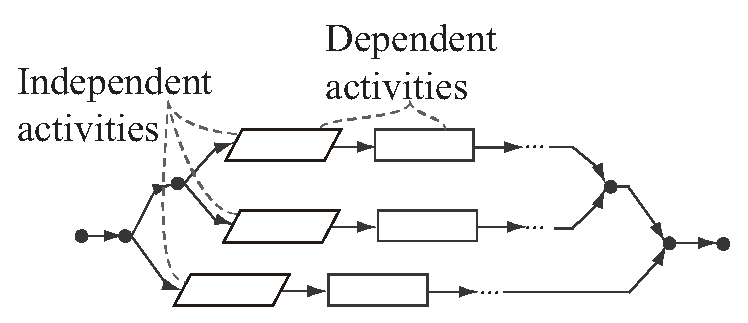
\epsfig{file=Images/maxpar.eps,scale=0.4}\label{fig:impl:maxpar}}
				&\qquad\qquad{}&
				\subfloat[\parminus{} workflow]{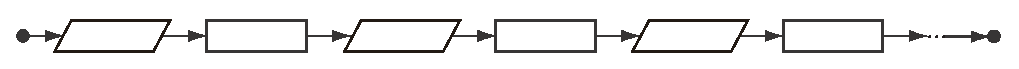
\epsfig{file=Images/maxseq.eps, scale=0.38}\label{fig:impl:maxseq}}			
		\end{tabular}
		\caption{Classification of alternative workflows}
		\label{fig:impl:workflowClassificationEx}
	\end{figure}

\vspace*{-0.3cm}

The generated workflows were classified by analyzing the data dependencies among activities and their structures.
A workflow whose independent activities are composed in parallel is classified as \maxpar{}, \cf{} Figure \ref{fig:impl:maxpar}; otherwise it is classified as \parminus{}, \cf{} Figure \ref{fig:impl:maxseq}.
The charts in Figure \ref{fig:impl:ssDFCF} show the search spaces with the classification of workflows and the required time for each ASASEL workflow $WF^{1},...,WF^{7}$.


	\begin{figure}
		\centering
		\begin{tabular}{lr}
				\subfloat[Clasification of the search spaces]{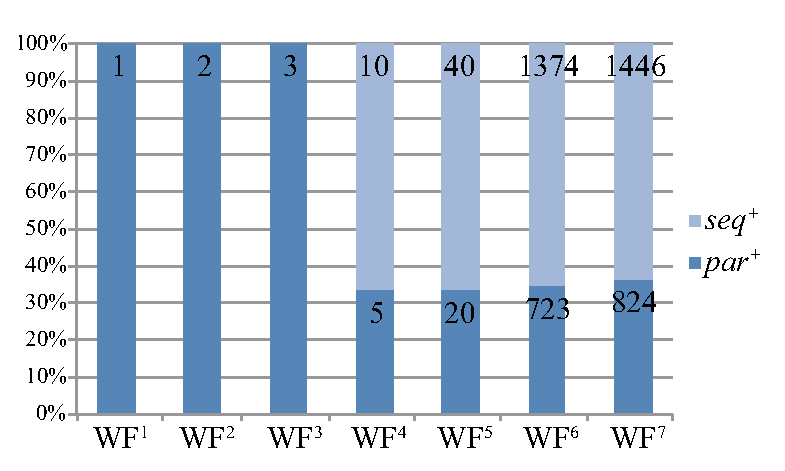
\epsfig{file=Images/ssClassification.eps,scale=0.5}	\label{fig:searchspaceClassification}}
				&
				\subfloat[Required time]{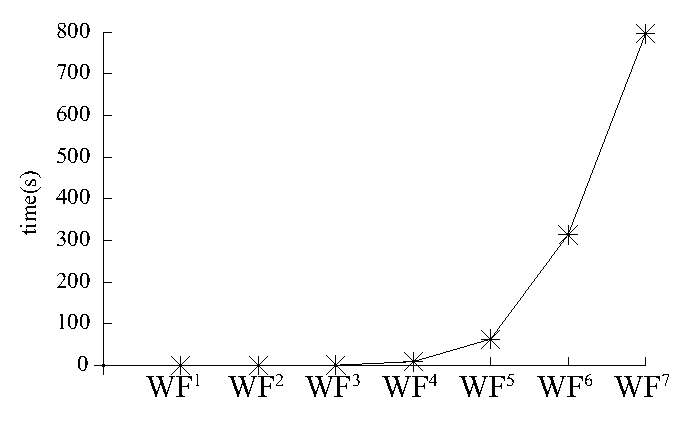
\epsfig{file=Images/time.eps, scale=0.5}\label{fig:timeGraph}}			
		\end{tabular}
		\caption{Enumeration of the space of alternative workflows with different grade of parallelism}
		\label{fig:impl:ssDFCF}
	\end{figure}
				
In Figure \ref{fig:searchspaceClassification}, the search spaces of the workflows $WF^{1}-WF^{3}$ only contain \maxpar{} workflows because they have few activities and there are no independent activities.
The search spaces of the workflows $WF^{4}-WF^{7}$ have $\sim${}1/3 of \maxpar{} workflows and $\sim$2/3 \parminus{} workflows. 
This correspondence is not constant and depends on the data dependencies among activities, \eg{} a workflow with many activities may have only sequential alternatives if there are no independent activities.

The \maxpar{} workflows represent good opportunities for improving time related costs while the \parminus{} ones privilege the resource usage.
This classification can be used for improving the enumeration performance (\cf{} Figure \ref{fig:timeGraph}) by incorporating user's preferences over the costs or QoS measures associated to the workflow execution.

 
%%\vspace*{1cm}
%%
%%
%%We defined four workflow cases with different number of required activities based on the example of Section \ref{subsec:kb}. We performed experiments for measuring the size of the search space given the expected length of workflows. The length determines the size of the search space and thus the required time to perform the transformation. We used lengths from 6 to 14.
%%
%%The growth of the search space is shown in Figure \ref{fig:graphs}. The size tends to be stable once it has reached the maximum length with all the required activities composed in sequence. For instance, $W1$ has $11$ required activities and it reaches the maximum length with $l=11$. The workflows with the "maximum" number of parallel compositions are the ones with the small $l$. For instance with $l=7$, $W1$ has the maximum number of parallel compositions\footnote{See http://goo.gl/XKZuL and http://goo.gl/z4iu3 for examples of lengths 7 and 11.}.
%%
%%%\tabsize{tab:size}{Search space growth respect to the plan length}
%%
%%%\tabtime{tab:time}{Time for workflow transformations with different lengths}
%%
%%\begin{figure*}
%%	\centering
%%		\begin{tabular}{lr}
%%%				\subfloat[Search space]{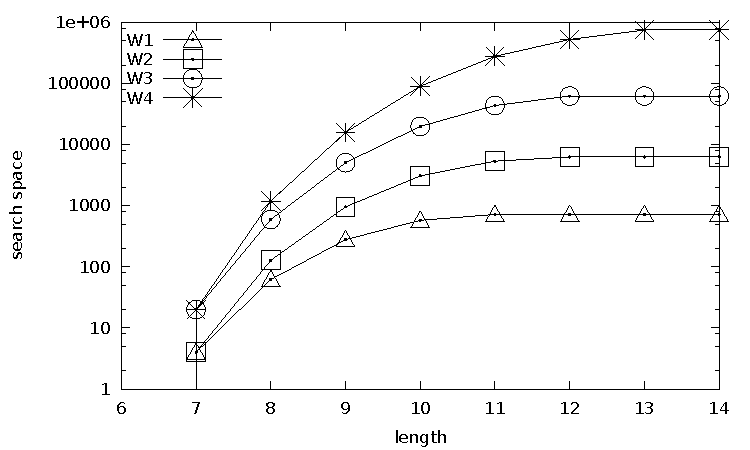
\epsfig{file=Images/searchspace.pdf, scale=0.47}\label{fig:searchspaceGraph}}
%%				&
%%%				\subfloat[Execution time]{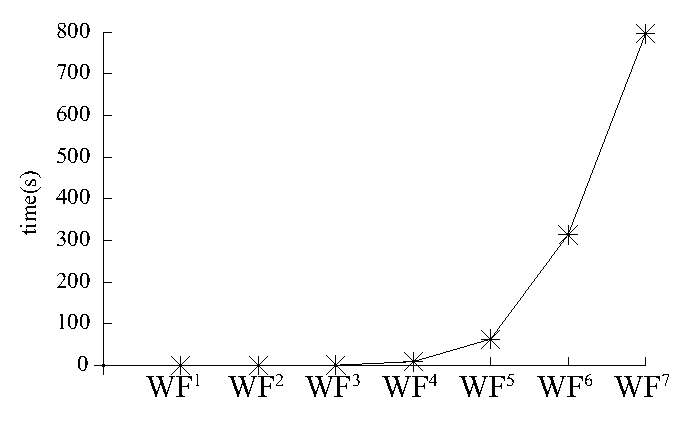
\epsfig{file=Images/time.eps, scale=0.47}\label{fig:timeGraph}}			
%%		\end{tabular}
%%		\caption{Search space and execution time}
%%		\label{fig:graphs}
%%\end{figure*}
%%
%%Besides the size of search space, the time for processing the workflow generation is exponential (\cf{} Figure \ref{fig:graphs}) and it is not feasible to generate completely the search space. Future work involves exploring alternative encodings and planning systems to obtain better performance.

